\documentclass{standalone}
\usepackage{tikz}
\usetikzlibrary{patterns, positioning}
\usepackage[sfdefault]{ClearSans} %% option 'sfdefault' activates Clear Sans as the default text font
\usepackage[T1]{fontenc}

\begin{document}
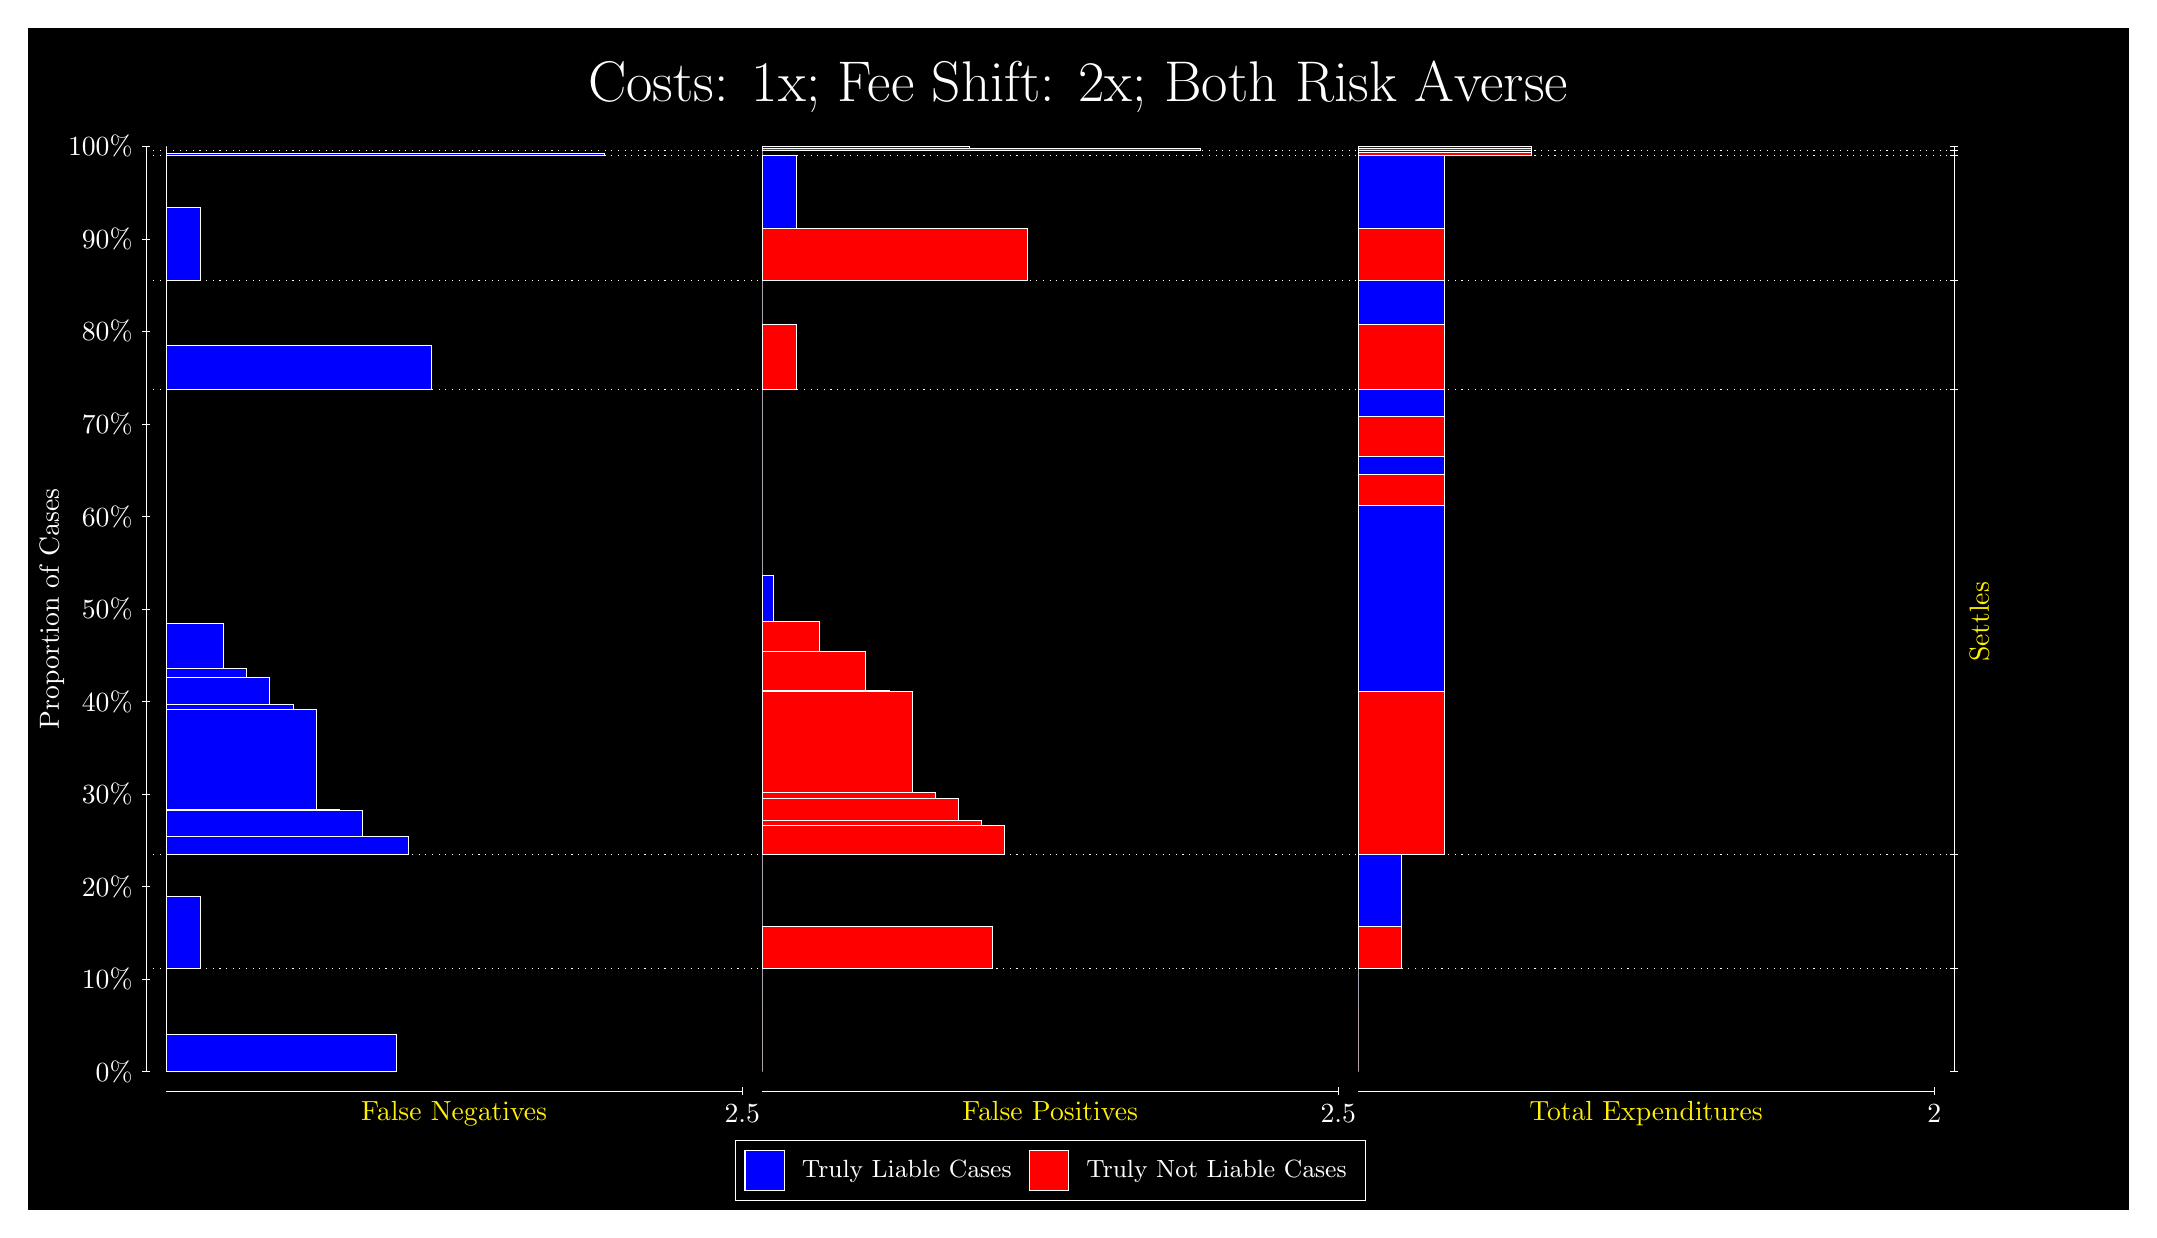
\begin{tikzpicture}
\draw[fill=black] (0,0) rectangle (26.667,15);
\draw[text=white] (0,13.5) rectangle (26.667,15) node[midway] {\huge Costs: 1x; Fee Shift: 2x; Both Risk Averse};
\draw[white, very thin] (1.5,1.75) -- (1.5,13.5);
\node[rotate=90, text=white, anchor=center] at (0.3, 7.625) {Proportion of Cases};
\draw[white, very thin] (1.45,1.75) -- (1.55,1.75);
\node[text=white, anchor=east] at (1.45, 1.75) {0\%};
\draw[white, very thin] (1.45,2.925) -- (1.55,2.925);
\node[text=white, anchor=east] at (1.45, 2.925) {10\%};
\draw[white, very thin] (1.45,4.1) -- (1.55,4.1);
\node[text=white, anchor=east] at (1.45, 4.1) {20\%};
\draw[white, very thin] (1.45,5.275) -- (1.55,5.275);
\node[text=white, anchor=east] at (1.45, 5.275) {30\%};
\draw[white, very thin] (1.45,6.45) -- (1.55,6.45);
\node[text=white, anchor=east] at (1.45, 6.45) {40\%};
\draw[white, very thin] (1.45,7.625) -- (1.55,7.625);
\node[text=white, anchor=east] at (1.45, 7.625) {50\%};
\draw[white, very thin] (1.45,8.8) -- (1.55,8.8);
\node[text=white, anchor=east] at (1.45, 8.8) {60\%};
\draw[white, very thin] (1.45,9.975) -- (1.55,9.975);
\node[text=white, anchor=east] at (1.45, 9.975) {70\%};
\draw[white, very thin] (1.45,11.15) -- (1.55,11.15);
\node[text=white, anchor=east] at (1.45, 11.15) {80\%};
\draw[white, very thin] (1.45,12.325) -- (1.55,12.325);
\node[text=white, anchor=east] at (1.45, 12.325) {90\%};
\draw[white, very thin] (1.45,13.5) -- (1.55,13.5);
\node[text=white, anchor=east] at (1.45, 13.5) {100\%};

\draw[white, very thin] (24.457,1.75) -- (24.457,13.5);
\draw[white, very thin] (24.407,1.75) -- (24.507,1.75);
\node[anchor=west] at (24.407, 1.75) {};
\draw[white, very thin] (24.407,3.062) -- (24.507,3.062);
\node[anchor=west] at (24.407, 3.062) {};
\draw[white, very thin] (24.407,4.5042) -- (24.507,4.5042);
\node[anchor=west] at (24.407, 4.5042) {};
\draw[white, very thin] (24.407,10.416) -- (24.507,10.416);
\node[anchor=west] at (24.407, 10.416) {};
\draw[white, very thin] (24.407,11.799) -- (24.507,11.799);
\node[anchor=west] at (24.407, 11.799) {};
\draw[white, very thin] (24.407,13.384) -- (24.507,13.384);
\node[anchor=west] at (24.407, 13.384) {};
\draw[white, very thin] (24.407,13.446) -- (24.507,13.446);
\node[anchor=west] at (24.407, 13.446) {};
\draw[white, very thin] (24.407,13.5) -- (24.507,13.5);
\node[anchor=west] at (24.407, 13.5) {};

\draw[white, very thin, fill=blue] (1.75,1.75) rectangle (4.6775,2.2292);
\draw[white, very thin, fill=red] (1.75,2.2292) rectangle (1.75,3.062);
\draw[white, very thin, fill=blue] (1.75,3.062) rectangle (2.1891,3.9718);
\draw[white, very thin, fill=red] (1.75,3.9718) rectangle (1.75,4.5042);
\draw[white, very thin, fill=blue] (1.75,4.5042) rectangle (4.8239,4.7381);
\draw[white, very thin, fill=blue] (1.75,4.7381) rectangle (4.2384,5.0679);
\draw[white, very thin, fill=blue] (1.75,5.0679) rectangle (3.9457,5.0783);
\draw[white, very thin, fill=blue] (1.75,5.0783) rectangle (3.6529,6.354);
\draw[white, very thin, fill=blue] (1.75,6.354) rectangle (3.3602,6.415);
\draw[white, very thin, fill=blue] (1.75,6.415) rectangle (3.0674,6.7547);
\draw[white, very thin, fill=blue] (1.75,6.7547) rectangle (2.7746,6.8675);
\draw[white, very thin, fill=blue] (1.75,6.8675) rectangle (2.4819,7.4468);
\draw[white, very thin, fill=red] (1.75,7.4468) rectangle (1.75,10.416);
\draw[white, very thin, fill=blue] (1.75,10.416) rectangle (5.1167,10.973);
\draw[white, very thin, fill=red] (1.75,10.973) rectangle (1.75,11.799);
\draw[white, very thin, fill=blue] (1.75,11.799) rectangle (2.1891,12.729);
\draw[white, very thin, fill=red] (1.75,12.729) rectangle (1.75,13.384);
\draw[white, very thin, fill=blue] (1.75,13.384) rectangle (7.3123,13.411);
\draw[white, very thin, fill=red] (1.75,13.411) rectangle (1.75,13.446);
\draw[white, very thin, fill=red] (1.75,13.446) rectangle (1.75,13.47);
\draw[white, very thin, fill=blue] (1.75,13.47) rectangle (1.75,13.5);
\draw[white, very thin, fill=red] (9.3189,1.75) rectangle (9.3189,2.5829);
\draw[white, very thin, fill=blue] (9.3189,2.5829) rectangle (9.3189,3.062);
\draw[white, very thin, fill=red] (9.3189,3.062) rectangle (12.246,3.5945);
\draw[white, very thin, fill=blue] (9.3189,3.5945) rectangle (9.3189,4.5042);
\draw[white, very thin, fill=red] (9.3189,4.5042) rectangle (12.393,4.8769);
\draw[white, very thin, fill=red] (9.3189,4.8769) rectangle (12.1,4.9411);
\draw[white, very thin, fill=red] (9.3189,4.9411) rectangle (11.807,5.2167);
\draw[white, very thin, fill=red] (9.3189,5.2167) rectangle (11.515,5.3001);
\draw[white, very thin, fill=red] (9.3189,5.3001) rectangle (11.222,6.5753);
\draw[white, very thin, fill=red] (9.3189,6.5753) rectangle (10.929,6.5865);
\draw[white, very thin, fill=red] (9.3189,6.5865) rectangle (10.636,7.0816);
\draw[white, very thin, fill=red] (9.3189,7.0816) rectangle (10.051,7.4733);
\draw[white, very thin, fill=blue] (9.3189,7.4733) rectangle (9.4652,8.0525);
\draw[white, very thin, fill=blue] (9.3189,8.0525) rectangle (9.3189,10.416);
\draw[white, very thin, fill=red] (9.3189,10.416) rectangle (9.758,11.242);
\draw[white, very thin, fill=blue] (9.3189,11.242) rectangle (9.3189,11.799);
\draw[white, very thin, fill=red] (9.3189,11.799) rectangle (12.686,12.454);
\draw[white, very thin, fill=blue] (9.3189,12.454) rectangle (9.758,13.384);
\draw[white, very thin, fill=red] (9.3189,13.384) rectangle (9.3189,13.419);
\draw[white, very thin, fill=blue] (9.3189,13.419) rectangle (9.3189,13.446);
\draw[white, very thin, fill=red] (9.3189,13.446) rectangle (14.881,13.47);
\draw[white, very thin, fill=blue] (9.3189,13.47) rectangle (11.954,13.5);
\draw[white, very thin, fill=red] (16.888,1.75) rectangle (16.888,2.5829);
\draw[white, very thin, fill=blue] (16.888,2.5829) rectangle (16.888,3.062);
\draw[white, very thin, fill=red] (16.888,3.062) rectangle (17.437,3.5945);
\draw[white, very thin, fill=blue] (16.888,3.5945) rectangle (17.437,4.5042);
\draw[white, very thin, fill=red] (16.888,4.5042) rectangle (17.986,6.5753);
\draw[white, very thin, fill=blue] (16.888,6.5753) rectangle (17.986,8.9438);
\draw[white, very thin, fill=red] (16.888,8.9438) rectangle (17.986,9.3354);
\draw[white, very thin, fill=blue] (16.888,9.3354) rectangle (17.986,9.5693);
\draw[white, very thin, fill=red] (16.888,9.5693) rectangle (17.986,10.076);
\draw[white, very thin, fill=blue] (16.888,10.076) rectangle (17.986,10.416);
\draw[white, very thin, fill=red] (16.888,10.416) rectangle (17.986,11.242);
\draw[white, very thin, fill=blue] (16.888,11.242) rectangle (17.986,11.799);
\draw[white, very thin, fill=red] (16.888,11.799) rectangle (17.986,12.454);
\draw[white, very thin, fill=blue] (16.888,12.454) rectangle (17.986,13.384);
\draw[white, very thin, fill=red] (16.888,13.384) rectangle (19.083,13.419);
\draw[white, very thin, fill=blue] (16.888,13.419) rectangle (19.083,13.446);
\draw[white, very thin, fill=red] (16.888,13.446) rectangle (19.083,13.47);
\draw[white, very thin, fill=blue] (16.888,13.47) rectangle (19.083,13.5);
\draw[white, dotted] (1.5,3.062) -- (24.457,3.062);
\draw[white, dotted] (1.5,4.5042) -- (24.457,4.5042);
\draw[white, dotted] (1.5,10.416) -- (24.457,10.416);
\draw[white, dotted] (1.5,11.799) -- (24.457,11.799);
\draw[white, dotted] (1.5,13.384) -- (24.457,13.384);
\draw[white, dotted] (1.5,13.446) -- (24.457,13.446);
\draw[white, very thin] (1.75,1.5) -- (9.0689,1.5);
\node[text=yellow, anchor=north] at (5.4094, 1.5) {False Negatives};
\draw[white, very thin] (9.0689,1.45) -- (9.0689,1.55);
\node[text=white, anchor=north] at (9.0689, 1.45) {2.5};

\draw[white, very thin] (9.3189,1.5) -- (16.638,1.5);
\node[text=yellow, anchor=north] at (12.978, 1.5) {False Positives};
\draw[white, very thin] (16.638,1.45) -- (16.638,1.55);
\node[text=white, anchor=north] at (16.638, 1.45) {2.5};

\draw[white, very thin] (16.888,1.5) -- (24.207,1.5);
\node[text=yellow, anchor=north] at (20.547, 1.5) {Total Expenditures};
\draw[white, very thin] (24.207,1.45) -- (24.207,1.55);
\node[text=white, anchor=north] at (24.207, 1.45) {2};



\node[text=yellow, centered, rotate=90] at (24.777, 7.46) {Settles};





\draw (12.978300999999998,1.5) node[draw=none] (baseCoordinate) {};
\begin{scope}[align=center]
        \matrix[scale=0.5, draw=white, below=0.5cm of baseCoordinate, nodes={draw}, column sep=0.1cm]{
            \node[rectangle, draw, minimum width=0.5cm, minimum height=0.5cm, fill=blue] {}; &
            \node[draw=none, font=\small, text=white] (B) {Truly Liable Cases}; &
            \node[rectangle, draw, minimum width=0.5cm, minimum height=0.5cm, fill=red] {}; &
            \node[draw=none, font=\small, text=white] (B) {Truly Not Liable Cases}; \\
            };
\end{scope}

\end{tikzpicture}
\end{document}